\documentclass[11pt]{beamer}
%\usetheme{Pittsburgh}
\usepackage[utf8]{inputenc}
\usepackage[english]{babel}
\usepackage{amsmath}
\usepackage{amsfonts}
\usepackage{tikz}
\usetikzlibrary{shapes,arrows}
\usepackage{amssymb}
\author{Jonas Ackermann and Lasse Schuirmann}
\title{Discrete Inverse Problems - Solving Real Problems}
%\setbeamercovered{transparent} 
%\setbeamertemplate{navigation symbols}{} 
%\logo{} 
%\institute{} 
\date{19.09.2014} 
%\subject{}
\begin{document}
% Styles for diagram
\tikzstyle{decision} = [diamond, draw, fill=blue!20, 
    text width=4.5em, text badly centered, node distance=3cm, inner sep=0pt]
\tikzstyle{block} = [rectangle, draw, fill=blue!20, 
    text width=5em, text centered, rounded corners, minimum height=4em]
\tikzstyle{line} = [draw, -latex']
\tikzstyle{cloud} = [draw, ellipse,fill=red!20, node distance=3cm,
    minimum height=2em]

\begin{frame}
\titlepage
\end{frame}


\begin{frame}
\tableofcontents
\end{frame}


\begin{frame}{Barcode Reader}
\begin{center}

\includegraphics[scale=0.5]{Barcode_example.PNG} 
\end{center}
\end{frame}


\begin{frame}{Barcode Reader}
\begin{center}
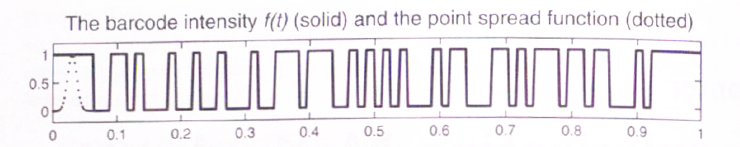
\includegraphics[scale=0.5]{Barcode_f.PNG} 
\end{center}
\end{frame}


\begin{frame}{Modellierung des Barcode Readers (1)}
\begin{center}
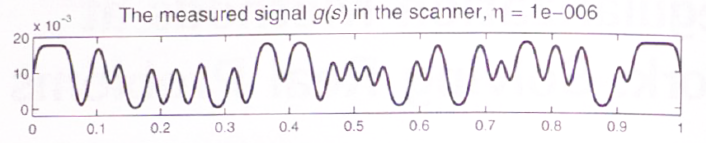
\includegraphics[scale=0.5]{Barcode_g.PNG} 
\end{center}
\end{frame}


\begin{frame}{Modellierung des Barcode Readers (2)}
\[g(s) = \int\limits_{0}^1 f(t) \cdot h(s-t) dt = \int\limits_{0}^1 f(t) \cdot e^{-\left(s-t \over \varsigma\right)^2} dt, \, \, \, \, \, \, 0 \leq s \leq 1 \]
\end{frame}


\begin{frame}{Barcode Reader: Faltung}
\[
g(s) = \int\limits_{0}^1 f(t) \cdot h(s-t) dt
\]

Entspricht einer Faltung $\rightarrow$ Invers: Dekonvolution (Entfaltung)
\end{frame}


\begin{frame}{Barcode Reader: Diskretisierung}
\[
a_{ij} = K(s_i, t_j) = \frac{1}{n} e^{-\left(i-j \over \varsigma n\right)^2}, \,\,\,\,\, i,j = 1, ..., n
\]

\[\]

\[
\mbox{Mit: } s_i = \frac{(i- \frac{1}{2})}{n}, \,\,\,\, t_j = \frac{(j - \frac{1}{2})}{n}
\]
\end{frame}


\begin{frame}{Barcode Reader: Rekonstruktion}
\begin{center}
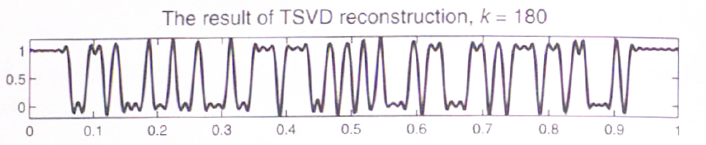
\includegraphics[scale=0.5]{Barcode_TSVD.PNG} 
\end{center}
\end{frame}


\begin{frame}{Data Model Mismatch (1)}

Modell basiert auf Annahmen über Daten. Annahmen erfüllt?

\end{frame}



\begin{frame}{Data Model Mismatch (2)}

\begin{center}

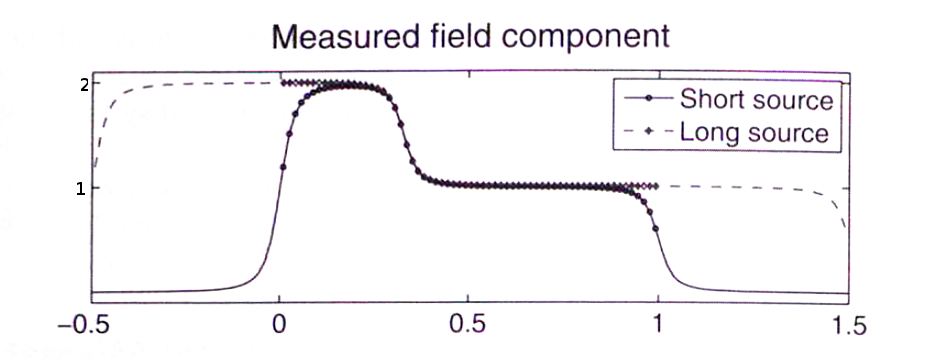
\includegraphics[scale=0.5]{DataModel_graph.PNG} 

\end{center}

\end{frame}


\begin{frame}{Inverse Crime (1)}
% TODO this should be more circular
\begin{tikzpicture}[node distance = 2cm, auto]
\node [cloud] (orig) {$f(t)$};
\node [block, right of=orig] (model) {Modell};
\node [cloud, right of=model] (blurred) {$g(s)$};
\node [block, below of=model] (inversemodel) {Inverses Modell};

\path [line] (orig) -- (model);
\path [line] (model) -- (blurred);
\path [line] (blurred) -- (inversemodel);
\path [line] (inversemodel) -- (orig);
\end{tikzpicture}

Kann das Modell anhand des Modells selbst geprüft werden?
\end{frame}



\begin{frame}{Inverse Crime (2)}

\begin{center}

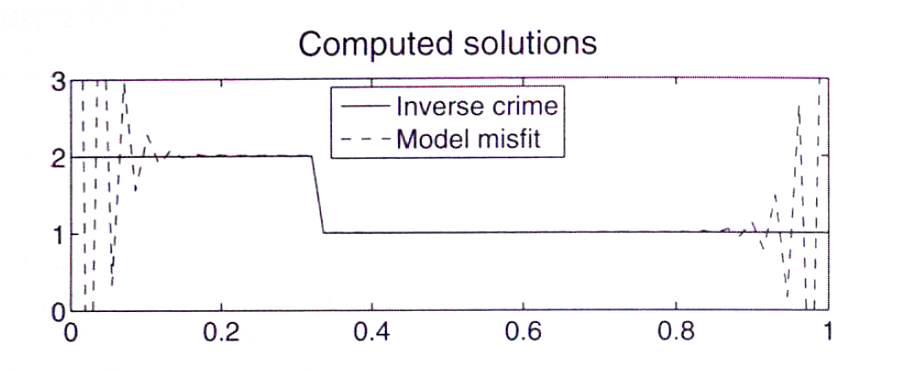
\includegraphics[scale=0.5]{InverseCrime.PNG} 

\end{center}

\end{frame}


\begin{frame}{Grenzbedingungen}

\end{frame}


\begin{frame}{Toeplitz Matrix}
\[
h[i-j] := a_{ij}
\]
\[
(x \star h)[i] = \sum\limits_{j=0}^{N-1} x[j] \cdot h[i-j] = b[i]
\]
\[
\begin{array}{c|cccc}
b[i]/x[j] & x[0] & x[1] & ... & x[N-1]  \\
\hline
b[0]     & h[0] & h[-1] & \cdots & h[-N+1] \\
b[1]     & h[1] & h[0] & \cdots & h[-N+2]  \\
\vdots  & \vdots & \vdots & \ddots & \vdots \\
b[N-1] & h[N-1] & h[N-2] & \cdots & h[0]  \\
\end{array}
\]
\end{frame}

\end{document}
